\chapter{ピクセルモジュール}
この章ではピクセルモジュールの構成と各構成部品について説明する。

\section{ピクセルモジュールの構成と信号伝達}
モジュールの構成を図\ref{module_configuration}に示す。
また、モジュールの信号伝達の様子を模式的に表したものを図\ref{module_electric_overview}に示す。

\begin{figure}[bpt]\centering
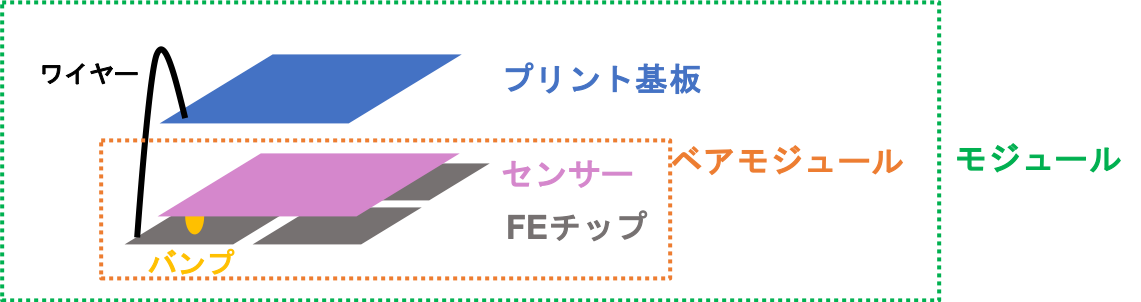
\includegraphics[width=14cm]{module_configuration}
\caption[ピクセルモジュールの構成]{ピクセルモジュールの構成}
\label{module_configuration}
\end{figure}

\begin{figure}[bpt]\centering
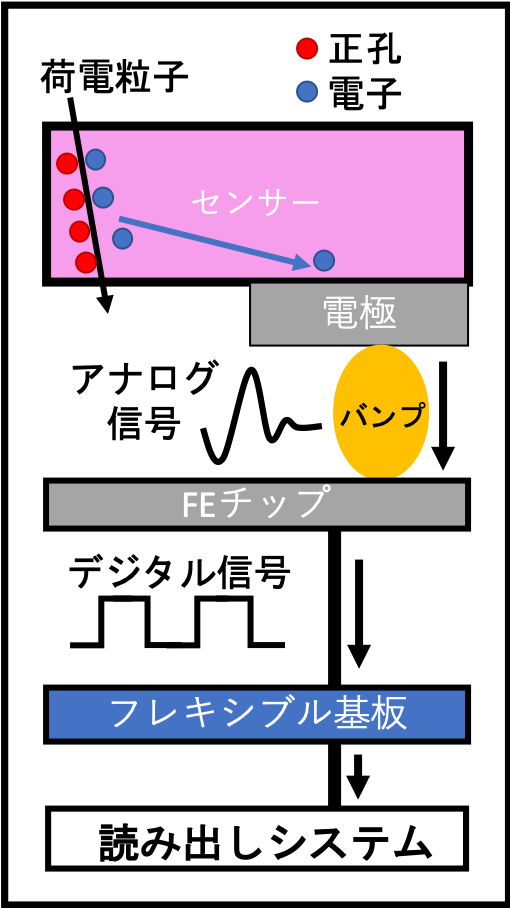
\includegraphics[width=8cm]{module_electric_overview}
\caption[ピクセルモジュールにおける信号伝達の様子]{ピクセルモジュールにおける信号伝達の様子}
\label{module_electric_overview}
\end{figure}

\section{ピクセルモジュールの構成部品}
\subsection{シリコンセンサー}
ピクセルモジュールに搭載するセンサーはシリコン半導体を用いている。
センサー内部にはpn接合\cite{2-1}を持つ。センサーに逆バイアス電極をかけ、空乏層\cite{2-1}を広げた状態で用いる。
この空乏層領域に荷電粒子が通過すると、Bethe-Blochの式\cite{2-1}に従い粒子はエネルギーを損失する。
このエネルギー損失量に従い、電子・ホール対が生成、これを収集することで荷電粒子の通過信号をアナログ信号として読み出すことができる。

新型ピクセルモジュールに搭載するセンサーでは、$n^+$ - in - p型を持つ。
模式図を図\ref{sensor_image}に示す。$n^+$電極で電子を収集し、信号取得を行う。
現行のセンサーに比べ、型変換を起こす可能性がなくなり安定した運転が見込まれる。\cite{1-3}

\begin{figure}[bpt]\centering
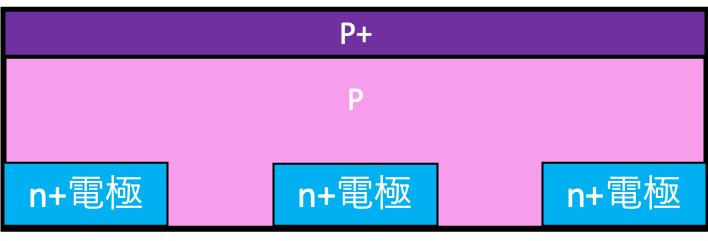
\includegraphics[width=8cm]{sensor_image}
\caption[センサーのイメージ]{センサーのイメージ}
\label{sensor_image}
\end{figure}

\subsection{読み出しFEチップ}
読み出しFEチップはシリコン半導体を用いて作られた集積回路である。
読み出しFEチップの主な役割は、シリコンセンサーで発生し受け取ったアナログ信号を整形、増幅したのちAD変換し、後段に転送することである。
AD変換について、アナログ信号がThresholdを超えた時間幅を測定し、デジタル信号に変換する。この信号の値を\textbf{Time over Threshold(ToT)}と呼ぶ。

このAD変換の流れのイメージを図\ref{tot_algorithm}に示す。

\begin{figure}[bpt]\centering
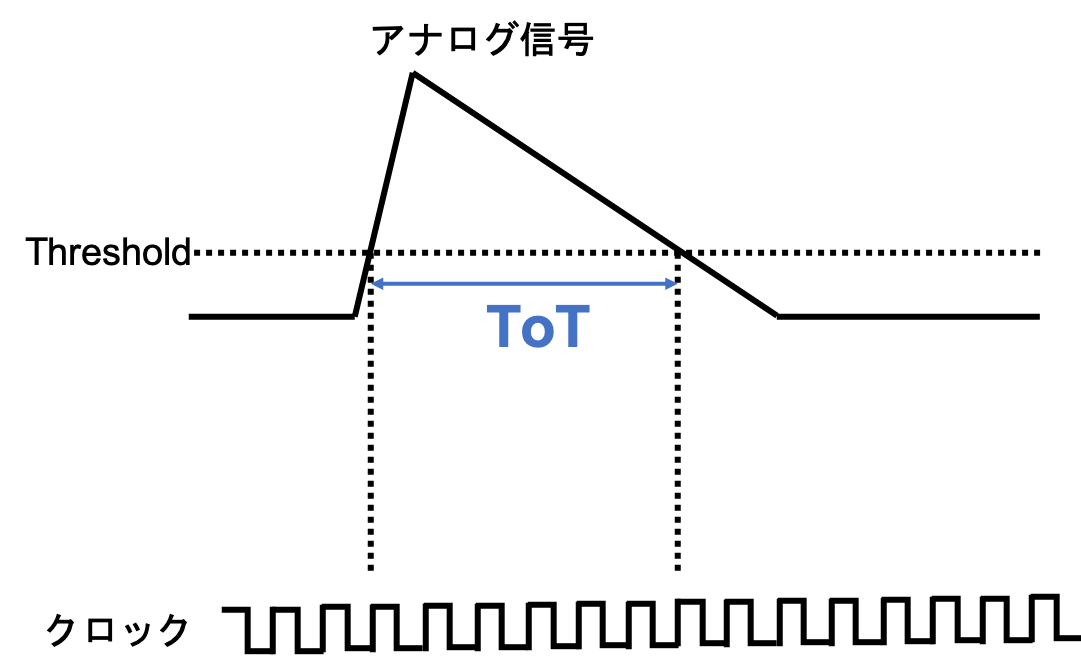
\includegraphics[width=10cm]{tot_algorithm}
\caption[ToTの概念図]{ToTの概念図}
\label{tot_algorithm}
\end{figure}



\subsubsection{RD53A}
RD53A\cite{2-1}は、新型ピクセルモジュールの研究、開発のために作られたプロトタイプの読み出しFEチップである。
RD53Aの性能を表\ref{rd53a_spec}に示す。
チップサイズ、ピクセル数はITkに搭載するモジュールの半分となっている。

\begin{table}[tbp]
\begin{center}
\caption[RD53Aの性能]{RD53Aの性能}
\label{rd53a_spec}
  \begin{tabular}{|ll|} \hline
    チップサイズ[mm$^2$] & $20.0\times 11.6$ \\ 
    ピクセルサイズ[$\mu$m$^2$] & $50.0\times 50.0$ \\ 
    ピクセル数[行$\times$列] & $400\times 192$ \\ 
    トリガーレート[kHz] & $1000$ \\ 
    データレート[Mbps] & $1280\times4$ \\ \hline
  \end{tabular}
\end{center}
\end{table}

FEチップ上の各ピクセルはアナログ回路部とデジタル回路部を持つ。
RD53Aでは図\ref{fechip_rd53a}に示すように、3つの領域があり、それぞれの領域でピクセルのアナログ回路部が異なる。
左から順にsynchronous、linier、differrentialと呼ぶ。
研究開発用に3つの領域が設けられており、ITkに搭載するモジュールにはDifferrentialフロントエンドを用いることが決定している。
なお、デジタル回路部は全てのピクセルにおいて共通である。
それぞれの回路図を付録\ref{chap:rd53a_circit}に示す。

\begin{figure}[bpt]\centering
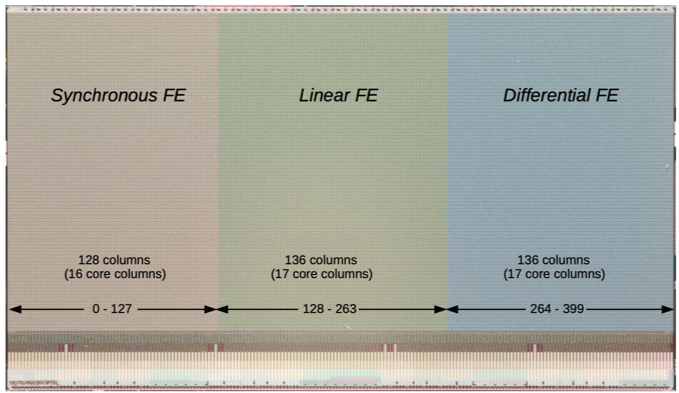
\includegraphics[width=10cm]{fechip_rd53a}
\caption[RD53A]{RD53A\cite{2-1}}
\label{fechip_rd53a}
\end{figure}

\subsection{フレキシブル基板}
フレキシブル基板は、基板上に電子部品が搭載されたものである。
FEチップからのデジタル信号を後段の回路へ転送する他、FEチップ、センサーへの電圧印加制御の役割も担う。

\section{新型モジュールの種類}
現在、ITkに搭載するモジュールとして以下の3つのモジュールを予定している。
\begin{itemize}
  \item ステーブ用Tripletモジュール
  \item リング用Tripletモジュール
  \item Quadモジュール
\end{itemize}

Triplet、QuadモジュールはそれぞれFEチップを3、4枚搭載するモジュールである。
それぞれのモジュールの図及び検出器上における位置の一例を図\ref{module_geom}に示す。

